\lecture{2}{29. Januar 2025}{Atomic structure}

\section{Introduction to atomic structure} \label{sec:int}
An atom consists of positively charged protons, negatively charged electrons and neutrally charged neutrons. In Bohr's model of the atom (\textbf{\autoref{fig:F2_1}}) the electrons are modelled ar orbiting a nucleus consisting of protons and neutrons. 
\begin{figure} [ht]
  \centering
  \caption{Bohr's model}
  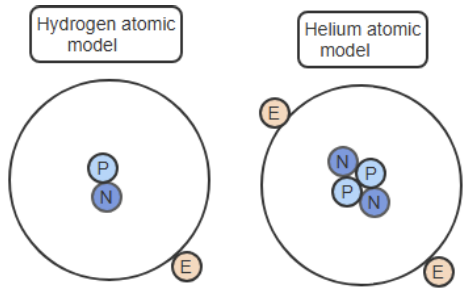
\includegraphics[width=0.35\linewidth]{./figures/F2_1.png}
  \label{fig:F2_1}
\end{figure}
Bohr's model was for a long time the commonly accepted atomic model in the scientific community, however we have come to believe that Bohr's notion of electrons being small particles in neatly defined orbits is over-simplified and that one instead should talk about an ``electron distribution''.

\subsection{Electron structure}
As mentioned in \autoref{sec:int} it turns out, that electrons have both particle-like and wave-like characteristics. Two of the wave like characteristics of electrons are that their position is given in terms of a Probability Density Function (PDF). The shape, size, and orientation of the PDF is given by the so called \textit{quantum numbers} (see \textbf{\autoref{fig:F2_2}}). The four quantum numbers are
\begin{figure} [ht]
  \centering
  \caption{The quantum numbers and how they relate.}
  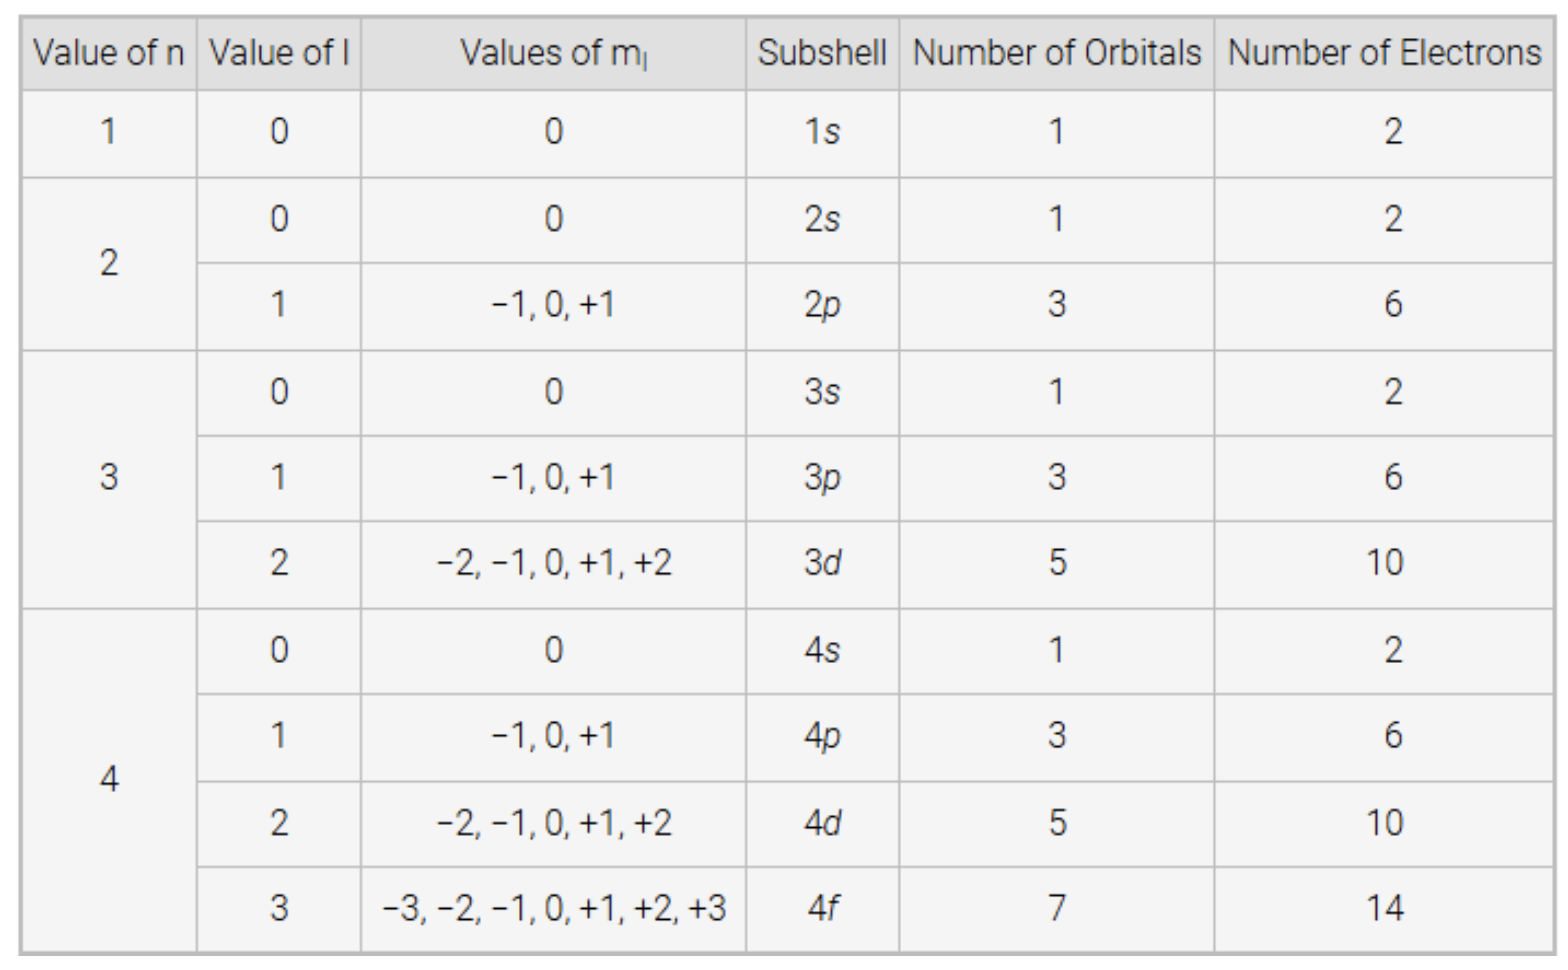
\includegraphics[width=0.65\linewidth]{./figures/F2_2.png}
  \label{fig:F2_2}
\end{figure}
\begin{itemize}
  \item $n = $ principal (shell) and is designated by $K, L, M, N, O (1, 2, 3, 4$,etc.)
  \item $l =$ azimuthal (subshell) and is designated by $s, p, d, f, (0, 1, 2, 3, \ldots n-1)$.
  \item $m_l = $ magnetic (no. of orbitals) and is designated by $-l$ to $l$.
  \item $m_s =$ spin and is either $-\frac{1}{2}$ or $\frac{1}{2}$.
\end{itemize}
Two electrons in the same atom cannot have the same quantum numbers as this violates Pauli's exclusion principle (PEP). The different subshells (azimuthal quantum number) have discrete energy values and they tend to occupy the lowest available energy-states (see \textbf{\autoref{fig:F2_3}}).
\begin{figure} [ht]
  \centering
  \caption{Discretization of the energy levels of the subshells.}
  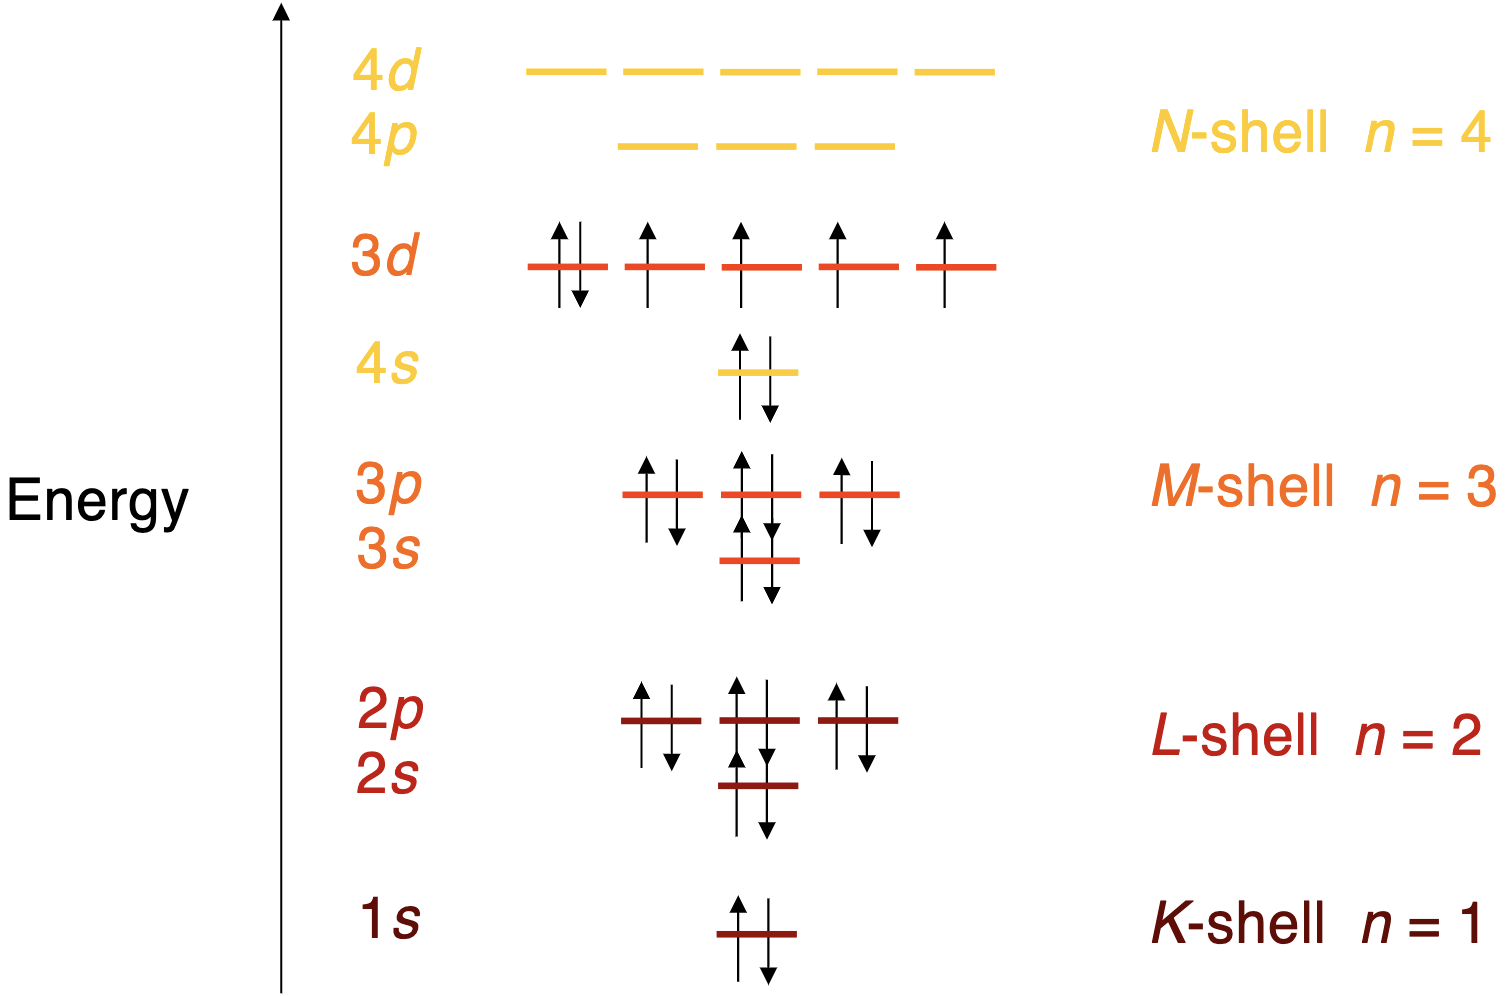
\includegraphics[width=0.55\linewidth]{./figures/F2_3.png}
  \label{fig:F2_3}
\end{figure}
The electrons in the outer unfilled shells are called \textit{valence electrons}. Valence electrons have a tendency to be more reactive than other electrons as it requires less energy to move an electron from an unfilled shell than from a filled shell. On \textbf{\autoref{fig:F2_3}} the valence electrons are $3d^6$ and $4s^2$. On \textbf{\autoref{fig:F2_4}} an illustration by Mikkel Klitgaard Nissen showcases how all of the above quantum numbers relate.
\begin{figure} [ht]
  \centering
  \caption{Illustration showcasing how the quantum numbers relate visually. By Mikkel Klitgaard Nissen.}
  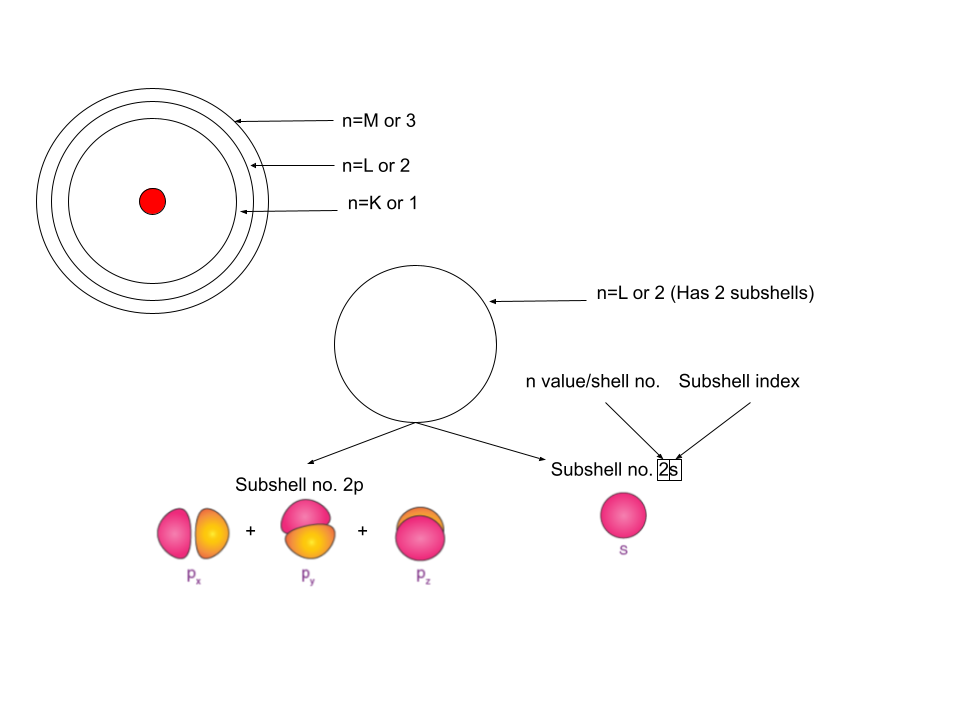
\includegraphics[width=0.55\linewidth]{./figures/F2_4.png}
  \label{fig:F2_4}
\end{figure}


\subsection{Trends in the periodic table}
Elements in each column of the periodic table have similar valence electron structure. In general the elements in the first column have 1 valence electron, the elements in the second column have 2 valence electrons and so on. Similarly the elements in the second-to-last column only need to gain 1 valence electron to fill their valence shell, whilst the elements in the last column already has a filled valence shell (the filled valence shell is the reason noble gasses are inert).

A quantified measure for the qualitative phenomenon above is \textit{electronegativity}. A small electronegativity translates to a tendency to lose electrons and a large electronegativity translates to a tendency to acquire electrons. All the elements and their electronegativity is shown in \textbf{\autoref{fig:F2_5}}.
\begin{figure} [ht]
  \centering
  \caption{The periodic table with electronegativity of each element shown.}
  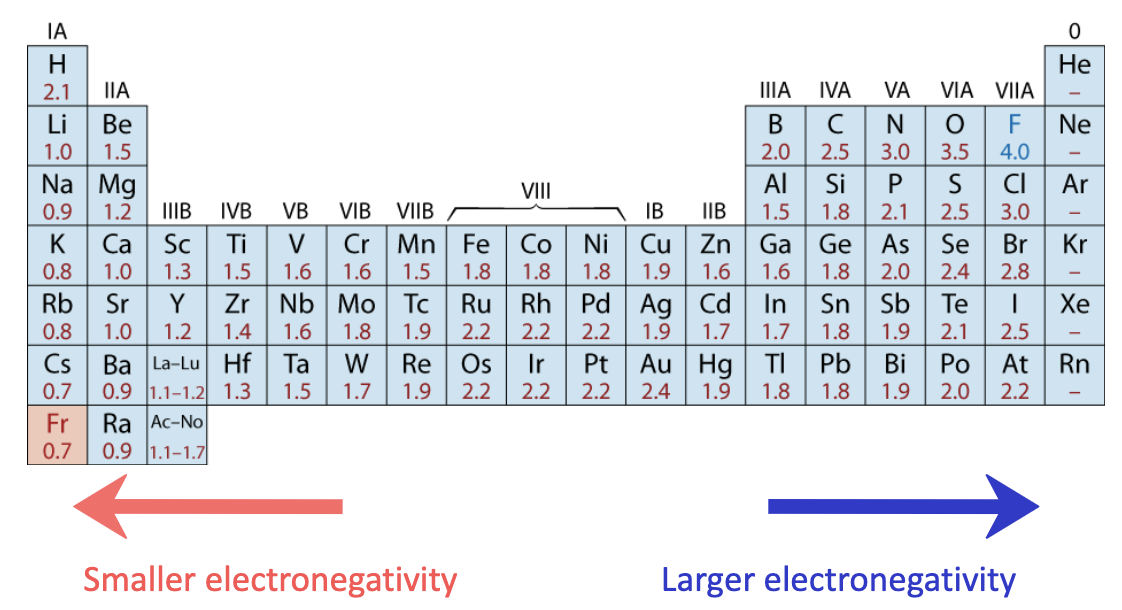
\includegraphics[width=0.8\linewidth]{./figures/F2_5.png}
  \label{fig:F2_5}
\end{figure}


\section{Bonding}
The interaction energy (potential energy) is shown as a function of seperation on \textbf{\autoref{fig:F2_6}}. This is also called the Coulomb interaction. As energy is the integral of the force a negative energy translates to an attractive force and vice-versa. The net potential energy is the sum of the repulsive and attractive energies. The repulsive energy has an asymptote at some $r > 0$ due to the PEP.
\begin{figure} [ht]
  \centering
  \caption{Potential energy as a function of seperation. Note $rn$ should be $r^n$, where $n \approx 6$.}
  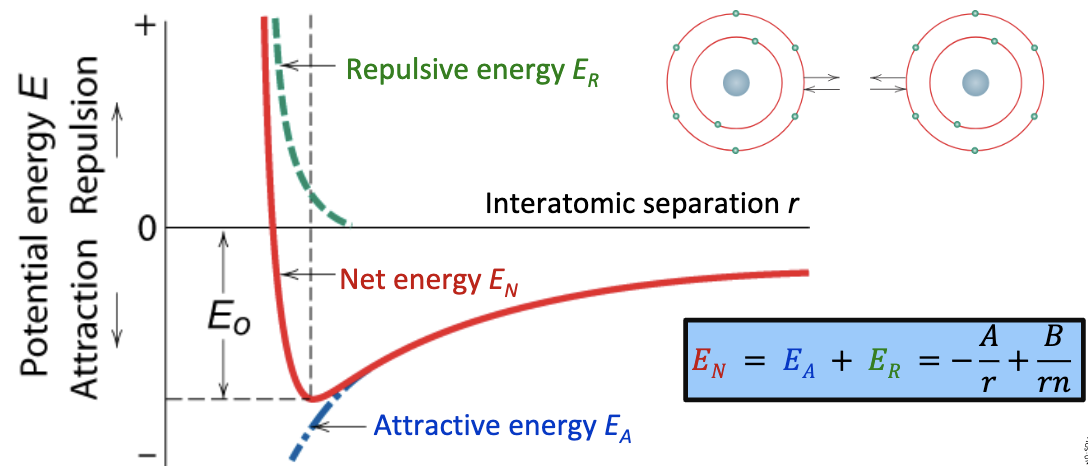
\includegraphics[width=0.75\linewidth]{./figures/F2_6.png}
  \label{fig:F2_6}
\end{figure}

\subsection{Ionic bonding}
Elements with dissimilar electronegativities gives rise to the phenomenon of \textit{ionization}. If one of the elements has a much larger ``interest'' in the electrons than the other then the other element will ``transfer'' one/some electron(s) to the first element. When the two elements have gained/lost an electron they have opposite charges and therefore an attractive electromagnetic interaction between them happens. A bond between atoms formed in this way is called an \textit{ionic bond}.

Ionic bonds are most off the time very strong and ionic bonding is the main bonding mechanism in ceramics.


\subsection{Covalent bonding}
Elements with similar electronegativities cannot pass electrons between them as easily as was the case for ionic bonding. Instead they have to ``share'' electrons. This is done in a way such that the two atoms each share one/some electron(s) so that the given electron(s) are in the valence shells of both atoms ``at once''. Normally it is the $s$ or $p$ orbitals that are involved. This bonding mechanism is called \textit{covalent bonding}.

\subsection{Metallic bonding}
In metals the electronegativity is normally rather low and therefore metals do not ``want'' to keep their valence electrons. Instead the electrons in a metal will form a de-localized electron ``cloud''. All of these free electrons are the reason metals are such good electrical conductors.


\subsection{Secondary bonding}
Other types of bonds than the above three also exist. These are called \textit{secondary bonds}. These are the weakest bonds but they are rather important as they give rise to phenomena such as adhesion. These types of bonds generally arise die to attractive forces between dipoles. 

\textit{Van der Waal's bonds} is the name for the bonding mechanism that happens due to randomly induced dipoles that come and go within the material at a rapid speed.

\textit{Hydrogen bonds} is the name for the phenomena that hydrogen covalently bound to a very electronegative atom has a tendency to bond make secondary bonds to other hydrogen atoms covalently bound to very electronegative atoms. This is for example the case in water where hydrogen is bound to the electronegative oxygen ($\sim\num{3,5}$).

\subsection{The relationship between bonding type, melting temperature and thermal expansion}
It is generally true, that the higher the bonding energy the higher the melting temperature. This is because more energy (heat) is required to break up a stronger bond (e.g. metallic) whereas less energy (heat) is required to break a weaker bond (e.g. polymer).

It is also generally true that the higher the bonding energy the lower the coefficient of thermal expansion. This is because an increase in the bond length ($\sim$coefficient of thermal expansion) leads to an assymetry in the attractive/repulsive energy curves and as the vonding energy increases this assymetry decreases.
